% =====================================================================
% Complete Figure Example: Skeleton B — 5-stage horizontal pipeline
% =====================================================================
% USAGE: Complete, COMPILABLE template for sub-agent to copy + customize.
% Strategy: BY-CONSTRUCTION — the 5 stages are chained with right=of (a
% single node distance), inter-stage arrows ride node anchors, and content
% labels wrap via text width. Change content, lengthen a label, or widen
% the hero and the rest REFLOWS automatically — no coordinate bookkeeping.
% (The old absolute-coordinate version lives in git history.)
%
% LAYOUT GRID (original design intent — now DERIVED by construction, not
% hand-typed; do not re-introduce absolute \node at (x,y)):
%   Stage 1: x=[0.0,  4.5],  y=[2,8]   Teal
%   Stage 2: x=[5.0,  9.5],  y=[2,8]   Blue
%   Stage 3: x=[10.0, 14.5], y=[2,8]   Purple (HERO)
%   Stage 4: x=[15.0, 19.5], y=[2,8]   Orange
%   Stage 5: x=[20.0, 24.5], y=[2,8]   Green
%   Bottom Summary Bar: y=[0.5, 1.2]
%   Bottom Color Legend: y=[-0.5, 0]
%
% Each stage uses SAME height = 6cm + same internal padding.
% Each stage = title strip (top 0.5cm) + content area (5.5cm).
%
% Sub-agent customization: change titles + labels + colors + numbers;
% the by-construction layout reflows. Do not hand-place absolute coords.
% =====================================================================

\documentclass[tikz,border=15pt]{standalone}
\usepackage{xcolor,tikz,amsmath,amssymb}
\usetikzlibrary{positioning,calc,backgrounds,arrows.meta,bending,fit}

\definecolor{acaBlueLine}{HTML}{3060A8}
\definecolor{acaBlueBg}{HTML}{DCE6F4}
\definecolor{acaPurpleLine}{HTML}{6E3FA0}
\definecolor{acaPurpleBg}{HTML}{EDE3F6}
\definecolor{acaOrangeLine}{HTML}{D06020}
\definecolor{acaOrangeBg}{HTML}{F9E0D0}
\definecolor{acaGreenLine}{HTML}{389050}
\definecolor{acaGreenBg}{HTML}{DBEDDC}
\definecolor{acaTealLine}{HTML}{1F8F8F}
\definecolor{acaTealBg}{HTML}{D3EBEB}
\definecolor{acaGreyLine}{HTML}{606060}
\definecolor{cellLo}{HTML}{F0E8F8}
\definecolor{cellHi}{HTML}{6E3FA0}

\pgfdeclarelayer{background}
\pgfsetlayers{background,main}

% ---- single source of truth for layout rhythm ----
\newlength{\stagew}\setlength{\stagew}{4.5cm}  % normal stage width
\newlength{\stageh}\setlength{\stageh}{6cm}     % stage height
\def\stagegap{0.5cm}                            % the ONE gap value

\tikzset{
  stage zone/.style={
    rectangle, rounded corners=4pt, line width=0.7pt,
    minimum width=\stagew, minimum height=\stageh, anchor=north west,
  },
  title strip/.style={
    anchor=north, font=\small\bfseries, text=white, rounded corners=2pt,
    inner ysep=2.5pt, yshift=-2pt, text width=3.9cm, align=center,
  },
  ibox/.style={  % internal content box: text width -> wraps, never overflows
    rectangle, rounded corners=3pt, line width=0.5pt, font=\scriptsize,
    align=center, inner sep=3pt, text width=3.2cm, minimum height=0.55cm,
  },
  flow arrow/.style={
    -{Stealth[length=5pt 1.2, width'=0pt 0.5]},
    line width=1.0pt, shorten >=2pt, shorten <=2pt, color=acaGreyLine,
  },
  node distance=\stagegap,
}

\begin{document}
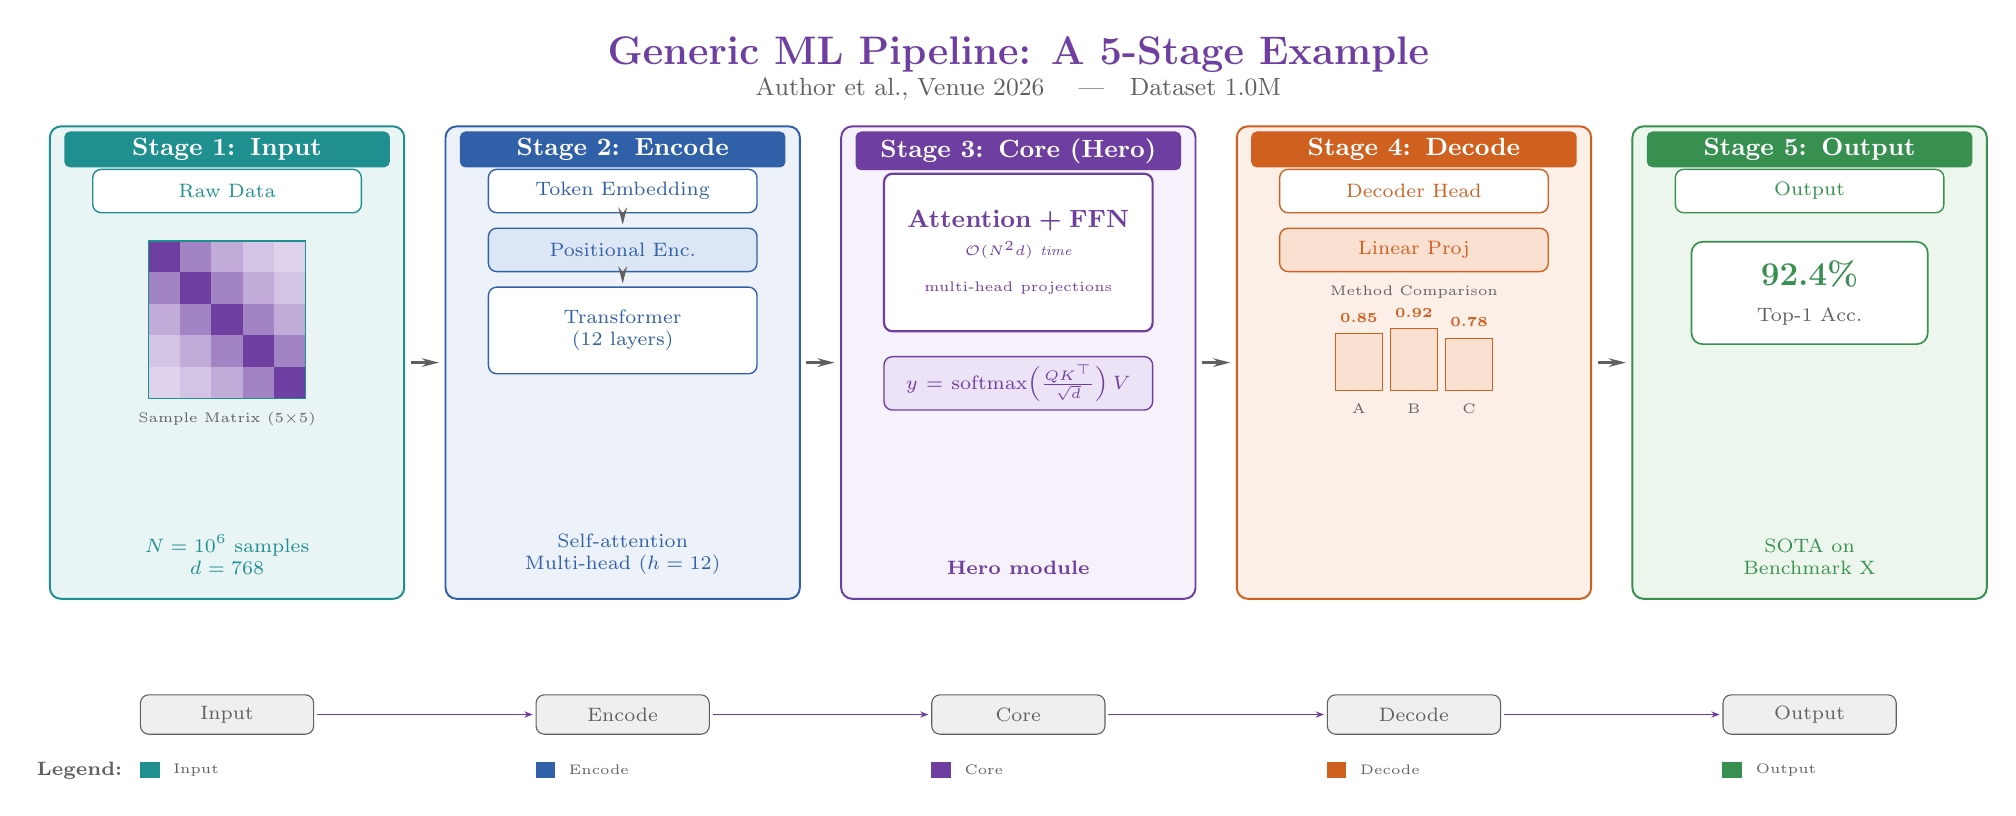
\begin{tikzpicture}

% =====================================================================
% STAGE ROW — first stage anchored, rest chained `right=of` previous
% =====================================================================
\node[stage zone, draw=acaTealLine]   (s1) at (0,0) {};
\node[stage zone, draw=acaBlueLine,   right=of s1] (s2) {};
\node[stage zone, draw=acaPurpleLine, right=of s2] (s3) {};  % HERO
\node[stage zone, draw=acaOrangeLine, right=of s3] (s4) {};
\node[stage zone, draw=acaGreenLine,  right=of s4] (s5) {};

% Zone backgrounds (behind everything)
\begin{pgfonlayer}{background}
  \fill[acaTealBg!50,  rounded corners=4pt] (s1.south west) rectangle (s1.north east);
  \fill[acaBlueBg!50,  rounded corners=4pt] (s2.south west) rectangle (s2.north east);
  \fill[acaPurpleBg!50,rounded corners=4pt] (s3.south west) rectangle (s3.north east);
  \fill[acaOrangeBg!50,rounded corners=4pt] (s4.south west) rectangle (s4.north east);
  \fill[acaGreenBg!50, rounded corners=4pt] (s5.south west) rectangle (s5.north east);
\end{pgfonlayer}

% Title strips (anchored to each stage .north -> follow the stage)
\node[title strip, fill=acaTealLine]   at (s1.north) {Stage 1: Input};
\node[title strip, fill=acaBlueLine]   at (s2.north) {Stage 2: Encode};
\node[title strip, fill=acaPurpleLine] at (s3.north) {Stage 3: Core (Hero)};
\node[title strip, fill=acaOrangeLine] at (s4.north) {Stage 4: Decode};
\node[title strip, fill=acaGreenLine]  at (s5.north) {Stage 5: Output};

% =====================================================================
% INTER-STAGE ARROWS — node anchors only. Cannot misalign under reflow.
% =====================================================================
\foreach \a/\b in {s1/s2, s2/s3, s3/s4, s4/s5} {
  \draw[flow arrow] (\a.east) -- (\b.west);
}

% =====================================================================
% STAGE 1 content — placed relative to s1 anchors
% =====================================================================
\node[ibox, fill=white, draw=acaTealLine, text=acaTealLine,
      below=0.55cm of s1.north] (s1_data) {Raw Data};
% heatmap centred under the data box, attached via scope shift to a node anchor
\begin{scope}[shift={($(s1_data.south)+(0,-1.35)$)}]
  \def\cs{0.4}\def\N{5}
  \foreach \i in {1,...,\N}\foreach \j in {1,...,\N}{
    \pgfmathsetmacro\val{int(exp(-abs(\i-\j)/2)*100)}
    \fill[cellHi!\val!cellLo]
      ({(\j-3)*\cs-\cs/2},{(3-\i)*\cs-\cs/2}) rectangle
      ({(\j-3)*\cs+\cs/2},{(3-\i)*\cs+\cs/2});
  }
  \draw[acaTealLine,line width=0.4pt]
    ({-\N*\cs/2},{-\N*\cs/2}) rectangle ({\N*\cs/2},{\N*\cs/2});
  \node[font=\tiny,color=acaGreyLine,anchor=north] at (0,{-\N*\cs/2-0.05})
    {Sample Matrix ($5{\times}5$)};
\end{scope}
\node[font=\scriptsize, color=acaTealLine, anchor=south, align=center]
  at ($(s1.south)+(0,0.2)$) {$N = 10^6$ samples\\$d = 768$};

% =====================================================================
% STAGE 2 content
% =====================================================================
\node[ibox, fill=white,    draw=acaBlueLine, text=acaBlueLine,
      below=0.55cm of s2.north] (s2_emb) {Token Embedding};
\node[ibox, fill=acaBlueBg, draw=acaBlueLine, text=acaBlueLine,
      below=0.18cm of s2_emb] (s2_pe) {Positional Enc.};
\node[ibox, fill=white,    draw=acaBlueLine, text=acaBlueLine,
      minimum height=1.1cm, below=0.18cm of s2_pe] (s2_tr) {Transformer\\(12 layers)};
\draw[flow arrow, shorten >=1pt, shorten <=1pt] (s2_emb.south) -- (s2_pe.north);
\draw[flow arrow, shorten >=1pt, shorten <=1pt] (s2_pe.south) -- (s2_tr.north);
\node[font=\scriptsize, color=acaBlueLine, anchor=south, align=center]
  at ($(s2.south)+(0,0.2)$) {Self-attention\\Multi-head ($h=12$)};

% =====================================================================
% STAGE 3 content (HERO)
% =====================================================================
\node[ibox, fill=white, draw=acaPurpleLine, text=acaPurpleLine, line width=0.8pt,
      minimum height=2.0cm, below=0.6cm of s3.north] (s3_hero)
  {{\small\bfseries Attention + FFN}\\[2pt]{\tiny\itshape $\mathcal{O}(N^2 d)$ time}\\[5pt]{\tiny multi-head projections}};
\node[ibox, fill=acaPurpleBg, draw=acaPurpleLine, text=acaPurpleLine,
      below=0.3cm of s3_hero] (s3_form)
  {$y = \text{softmax}\!\left(\frac{QK^\top}{\sqrt{d}}\right) V$};
\node[font=\scriptsize, color=acaPurpleLine, anchor=south]
  at ($(s3.south)+(0,0.2)$) {\textbf{Hero module}};

% =====================================================================
% STAGE 4 content
% =====================================================================
\node[ibox, fill=white,      draw=acaOrangeLine, text=acaOrangeLine,
      below=0.55cm of s4.north] (s4_dec) {Decoder Head};
\node[ibox, fill=acaOrangeBg, draw=acaOrangeLine, text=acaOrangeLine,
      below=0.18cm of s4_dec] (s4_lin) {Linear Proj};
% bar chart attached under the linear-proj box
\begin{scope}[shift={($(s4_lin.south)+(0,-1.5)$)}]
  \node[font=\tiny,color=acaGreyLine,anchor=south] at (0,1.05) {Method Comparison};
  \foreach \name/\val/\k in {A/0.85/-1, B/0.92/0, C/0.78/1}{
    \pgfmathsetmacro\bh{0.85*\val}
    \fill[acaOrangeBg] ({\k*0.7-0.3},0) rectangle ({\k*0.7+0.3},\bh);
    \draw[acaOrangeLine,line width=0.4pt] ({\k*0.7-0.3},0) rectangle ({\k*0.7+0.3},\bh);
    \node[font=\tiny\bfseries,color=acaOrangeLine,anchor=south] at (\k*0.7,\bh+0.02) {\val};
    \node[font=\tiny,color=acaGreyLine,anchor=north] at (\k*0.7,-0.05) {\name};
  }
\end{scope}

% =====================================================================
% STAGE 5 content
% =====================================================================
\node[ibox, fill=white, draw=acaGreenLine, text=acaGreenLine,
      below=0.55cm of s5.north] (s5_out) {Output};
\node[draw=acaGreenLine, fill=white, rounded corners=4pt, line width=0.6pt,
      minimum width=3.0cm, minimum height=1.3cm, align=center, inner sep=4pt,
      below=0.35cm of s5_out] (s5_metric)
  {{\large\bfseries\color{acaGreenLine} 92.4\%}\\[1pt]{\scriptsize\color{acaGreyLine} Top-1 Acc.}};
\node[font=\scriptsize, color=acaGreenLine, anchor=south, align=center]
  at ($(s5.south)+(0,0.2)$) {SOTA on\\Benchmark X};

% =====================================================================
% TITLE — centred on the whole row via calc midpoint (by construction)
% =====================================================================
\coordinate (rowtop) at ($(s1.north west)!0.5!(s5.north east)$);
\node[font=\Large\bfseries, color=acaPurpleLine, anchor=south]
  at ($(rowtop)+(0,0.55)$) {Generic ML Pipeline: A 5-Stage Example};
\node[font=\small, color=acaGreyLine, anchor=south]
  at ($(rowtop)+(0,0.2)$) {Author et al., Venue 2026 \quad|\quad Dataset 1.0M};

% =====================================================================
% SUMMARY BAR — one cell below each stage, then chained
% =====================================================================
\foreach \s/\lab in {s1/Input, s2/Encode, s3/Core, s4/Decode, s5/Output}{
  \node[rectangle, rounded corners=3pt, fill=acaGreyLine!10, draw=acaGreyLine,
        line width=0.4pt, font=\scriptsize, text=acaGreyLine, inner sep=4pt,
        minimum height=0.5cm, minimum width=2.2cm,
        below=1.2cm of \s.south] (sb-\s) {\lab};
}
\foreach \a/\b in {s1/s2, s2/s3, s3/s4, s4/s5}{
  \draw[-{Stealth[length=3pt]}, line width=0.5pt, color=acaPurpleLine,
        shorten >=1pt, shorten <=1pt] (sb-\a.east) -- (sb-\b.west);
}

% =====================================================================
% COLOR LEGEND — below the summary bar, tracks it
% =====================================================================
\node[font=\scriptsize\bfseries, color=acaGreyLine, anchor=east]
  at ($(sb-s1.south west)+(-0.1,-0.45)$) {Legend:};
\foreach \s/\col/\lab in {s1/acaTealLine/Input, s2/acaBlueLine/Encode,
      s3/acaPurpleLine/Core, s4/acaOrangeLine/Decode, s5/acaGreenLine/Output}{
  \fill[\col] ($(sb-\s.south west)+(0,-0.55)$) rectangle ($(sb-\s.south west)+(0.25,-0.35)$);
  \node[anchor=west, font=\tiny, color=acaGreyLine]
    at ($(sb-\s.south west)+(0.3,-0.45)$) {\lab};
}

\end{tikzpicture}
\end{document}
